\documentclass[a4paper]{article}
\usepackage[a4paper, top=17mm, bottom=17mm, left=17mm, right=17mm]{geometry}
\usepackage[utf8]{inputenc}
\usepackage[T2A,T1]{fontenc}
\usepackage[colorlinks,filecolor=blue,citecolor=green,unicode,pdftex]{hyperref}
\usepackage{cmap}
\usepackage[english,russian]{babel}
\usepackage{amsmath}
\usepackage{amssymb,amsfonts,textcomp}
\usepackage{color}
\usepackage{array}
\usepackage{hhline}
\hypersetup{colorlinks=true, linkcolor=blue, citecolor=blue, filecolor=blue, urlcolor=blue, pdftitle=1, pdfauthor=, pdfsubject=, pdfkeywords=}
\usepackage[pdftex]{graphicx}
\usepackage{graphicx}
% \usepackage{epigraph}
% Раскомментировать тем, у кого этот пакет есть. Шрифт станет заметно красивее.
%\usepackage{literat}
\usepackage{indentfirst}
\usepackage{multirow}
\usepackage{subfig}

\sloppy
\pagestyle{plain}
%\pagestyle{empty}

\title{Технология визуального предметно-ориентированного проектирования и разработки ПО QReal}

\author{А.Я.Кириленко \and Наталья Вальтман}
\date{}
\begin{document}

\maketitle
\thispagestyle{empty}

\begin{quote}
\small\noindent
абстракт
\end{quote}

\section*{Введение}

Модельно-ориентированная разработка ПО основывается на представлении программы в виде набора моделей, представляющих ее с различных точек зрения. При этом обычно используются визуальные языки моделирования, с их помощью создаются разного уровня абстракции описания предметной области, разрабатываемой системы и взаимодействующего с ней окружения. Считается, что в целом данный подход упрощает процесс разработки и понимания системы, делает его более наглядным. Наиболее активное распространение CASE-технологий [сноска] началось в середине 90-х годов прошлого века, когда появился унифицированный язык моделирования UML [ссылка]. К концу 90-х годов был разработан набор методологий разработки ПО (и поддерживающих их инструментариев), в том или ином виде предполагающих активное использование визуального проектирования. Среди них [примеры]. Однако, желание иметь полную автоматическую генерацию исполняемого кода по диаграммам неизбежно влечет к жесткой формализации соответствующих графических языков. При этом использование языков общего назначения чаще всего приводит к тому, что диаграммы теряют наглядность и простоту, становятся громоздкими и сложными для восприятия. Парадигма предметно-ориентированного моделирования же основывается на том факте, что чаще создание нового специального языка и решение с его помощью поставленной практической задачи можно осуществить быстрее, чем решать ту же задачу с помощью языков общего назначения. Имея соответствующую инструментальную поддержку, данный подход позволяет значительно повысить уровень абстракции, но котором работают проектировщики, и увеличить производительность их труда в несколько раз ([ссылки на статьи из Книжки]).

\section{Предыстория}

Разработкой технологии QReal занимается научно-исследовательская группа изучения технологий визуального моделирования кафедры системного программирования Санкт-Петербургского Государственного Университета. Проект QReal базируется на результатах, полученных на кафедре и в лаборатории системного программирования под руководством проф. А.Н. Терехова с 1984 года. Первые разработанные графические редакторы создавались для поддержки языка SDL (рекомендация МККТТ Z.100 [ссылки]), к концу 80-х годов была реализована генерация программ управления телефонными станциями, генерация баз данных и сложных форм ввода/вывода к ним — технология RTST [ссылки]. 

К середине 90-х годов группой была реализована поддержка появившегося в то время языка UML 1.4 в виде технологии REAL [ссылки]. Технология не создавалась как универсальная, а была ориентирована на создание информационных систем, ориентированных на данные (диаграммы классов, объектов, задание ограничений с помощью OCL), а также создания встроенных систем реального времени (диаграммы классов, последовательностей, конечных автоматов). 

Технология QReal [ссылки] изначально задумывалась как развитие технологии REAL, основывающееся на использовании более современной версии языка UML --- 2.0. При этом на разрабатываемые средства накладывались требования многоплатформенности (возможность работы на наиболее популярных операционных системах MS Windows и Linux), поддержка многопользовательской разработки, возможность удаленного доступа к репозиторию системы и другая актуальная для сред визуального проектирования ПО функциональность. Однако, очевидно, что создание большого числа редакторов диаграмм вручную является довольно утомительным занятием, к тому же получаемая система оказывается плохо масштабируемой --- создание дополнительного редактора, являющегося типовым для данного CASE-средства, чаще всего будет осуществляться методом Copy/Paste с дальнейшими доработками полученного после копирования, что влечет как к появлению дополнительных ошибок, связанных с неполнотой вносимых правок, так и к размножению уже существующих. В результате в QReal были добавлены средства метамоделирования, которые позволяют быстро создавать новые редакторы, описывания метамодель разрабатываемого языка и визуальное представление его элементов.

\section{QReal}

Инфраструктуру QReal можно представить следующим образом (см. рис.~\ref{qRealArchitecture}):

\begin{itemize}
  \item QReal имеет архитектуру «клиент-сервер» и основывается на шаблоне проектирования Model/View. Каждый клиент имеет свою модель, которая обеспечивает доступ к репозиторию, а в роли представлений выступают различные элементы пользовательского интерфейса (инспектор логических и графических моделей, редактор свойств и т.д.).
  \item Графический интерфейс QReal обычно содержит вполне определенный набор элементов: инспектор логических моделей, инспектор графических моделей, редактор свойств элементов, палитра компонентов, окно отображения ошибок и предупреждений, различные меню, панели инструментов, рабочая область графических редакторов диаграмм.
  \item Для обеспечения версионирования и многопользовательской работы используется сервер Subversion. Доступ к нему осуществляется посредством клиентов репозитория, которые хранят свои модели в виде файлов, организованных в рабочую копию системы контроля версий. При старте QReal файлы моделей читаются с диска и строится особая объектная структура, с которой и происходит работа при манипуляциями с репозиторием. При выходе из системы (либо по запросу пользователя) содержимое клиента репозитория может быть сериализовано на диск и внесенные изменения отправляются на SVN-сервер. В настоящее время в QReal поддержаны основные команды работы с subversion: commit, checkout, update. 
  \item Генераторы могут быть встроенными в клиентскую часть CASE-пакета (например, генератор XMI-описаний диаграмм [ссылка]) или работать независимо. В таком случае им потребуется компонента, отвечающая за взаимодействие с SVN-репозиторием и представление модели в памяти. Общение с ней ведётся по протоколу ICE [ссылка], что позволяет реализовывать генераторы на различных языках программирования.
  \item Ввиду того, что набор графических редакторов QReal не фиксирован, каждый визуальный редактор является подключаемым модулем. Инфраструктура CASE-системы включает в себя абстрактное ядро, реализующее общую для всех редакторов и элементов диаграмм функциональность, и подключаемых модулей, реализующих специфику конкретных редакторов. Каждый такой модуль инкапсулирует в себе информацию о наборе объектов, допустимых на диаграммах данного типа, позволяет правильно интерпретировать хранящиеся в репозитории значения атрибутов элементов (например, использовать некоторые из атрибутов как параметры при отрисовке элементов), предоствляет информацию о логических правилах размещения элементов на соответствующих типах диаграмм (например, возможность соединять некоторые элементы ассоциациями, возможность одних элементов быть контейнером для других и т.д.).
  \item Основная идея разделения логических и графических моделей состоит в том, что элемент модели и его визуальное представление --- по сути разные вещи. Некоторые элементы модели могут вовсе визуального представления не иметь (например, значения перечислимых типов или специальные служебные вещи типа настроек генерации), некоторые наоборот, имеют только визуальное представление и на логику никак не влияют (например, просто линия или прямоугольник на диаграмме), некоторые могут иметь несколько представлений (например, один и тот же класс UML может присутствовать на нескольких разных диаграммах, причём выглядеть по-разному). 
  \item Для некоторых видов поведенческих диаграмм в QReal реализован визуальный интерпретатор. 

\end{itemize}

\begin{figure} [ht]
  \begin{center}
    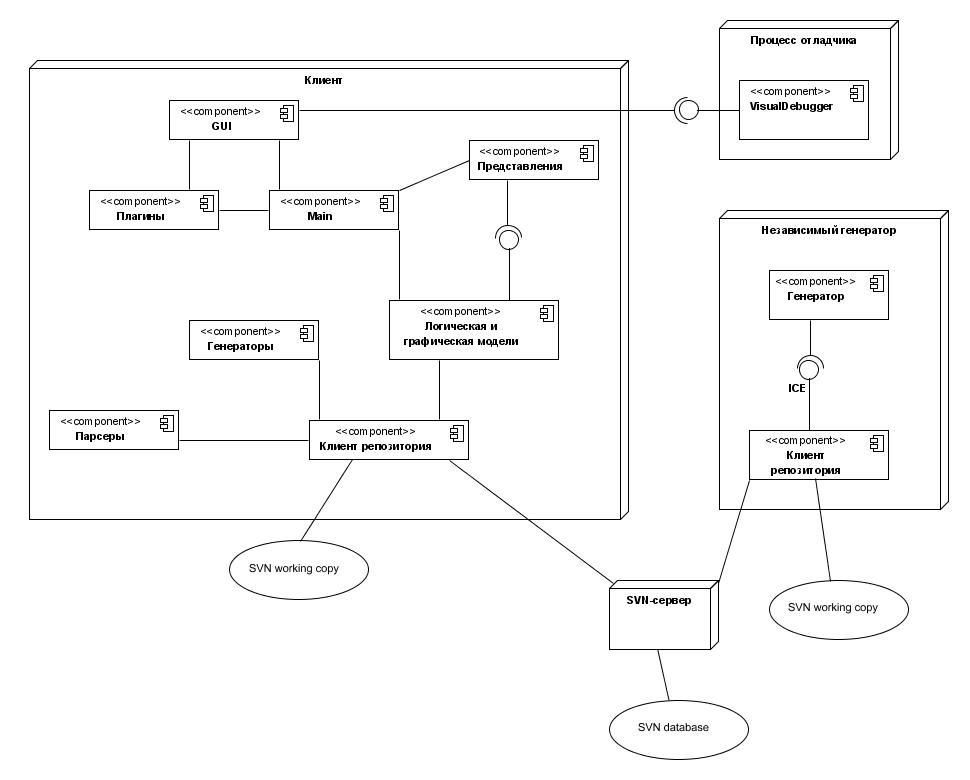
\includegraphics[width=0.9\textwidth]{01-architecture.png}
    \caption{Архитектура QReal}
    \label{qRealArchitecture}
  \end{center}
\end{figure}





\subsection{Средства метамоделирования}

В QReal реализованы два подхода, позволяющие любому заинтересованному пользователю системы, не обладающему навыками программирования и не знакомому с внутренним устройством системы, создать новый редактор диаграмм, встраивающийся в QReal.
\begin{itemize}
  \item Метамодель разрабатываемого языка описывается в виде XML-формата довольно простой структуры. Графические изображения элементов задаются с помощью текстового языка SDF, являющегося расширением языка описания векторной графики SVG [ссылка].
  \item Метамодель языка задается графически в метаредакторе QReal последством простого визуального языка, являющего аналогом MOF [ссылка]. Для описания представлений элементов языка на диаграммах используется графический редактор форм, позволяющий создавать из набора примитивов векторные изображения или загружать уже готовые растровые.
\end{itemize}








\subsection{Advanced usability}

\section{Заключение}



\end{document}